\documentclass{scrartcl}

\usepackage{tumbase}
\usepackage[colormodel=@COLORMODEL@]{tumcolors}

\usepackage{graphicx}

\newcommand{\crule}[1]{\textcolor{#1}{\rule{24mm}{6mm}}}


\title{The \texttt{tumcolors} package}
\author{\LaTeX4EI}
\date{09.08.2021}


\begin{document}

\maketitle


\begin{abstract}
  This package provides the colors defined by the TUM Corporate Design.
  All colors are defined for the colormodels rgb and cmyk. The required
  colormodel may be chosen by a package option.

  Where applicable, the corresponding \LaTeX\ standard colors are
  overwritten.
\end{abstract}


\section{Package dependencies}
The \texttt{tumcolors} package depends on the following list of \LaTeX\
packages.
\begin{itemize}
  \item xcolor (with table option)
  \item pgfkeys
  \item pgfopts
\end{itemize}


\section{Package options}
The \texttt{tumcolors} package provides the option \textbf{colormodel}, which
accepts the values \textbf{rgb} or \textbf{cmyk}. The option \textbf{print}
is a shorthand notation for the colormodel cmyk.
The default colormodel is rgb.

\begin{verbatim}
  \usepackage[colormodel=rgb]{tumcolors}
  \usepackage[colormodel=cmyk]{tumcolors}
  \usepackage[print]{tumcolors}
\end{verbatim}


\clearpage
\section{TUM corporate design colors}
This test case shows the TUM corporate design colors using the
\textbf{@COLORMODEL@} colormodel.

\subsection{Primary colors}
\begin{center}
  \begin{tabular}{cccc}
    \textbf{Color} &                  &               &
    \textbf{\LaTeX{} color}                             \\
    TUMBlue        & \crule{TUMBlue}  & \crule{blue}  &
    blue                                                \\
    TUMWhite       & \crule{TUMWhite} & \crule{white} &
    white                                               \\
    TUMBlack       & \crule{TUMBlack} & \crule{black} &
    black
  \end{tabular}
\end{center}

\subsection{Secondary colors}
\begin{center}
  \begin{tabular}{cccc}
    \textbf{Color} &                       &                   &
    \textbf{\LaTeX{} color}                                      \\
    TUMBlueDark    & \crule{TUMBlueDark}   &                   & \\
    TUMBlueDarker  & \crule{TUMBlueDarker} &                   & \\
    TUMGrayDark    & \crule{TUMGrayDark}   & \crule{darkgray}  &
    darkgray                                                     \\
    TUMGray        & \crule{TUMGray}       & \crule{gray}      &
    gray                                                         \\
    TUMGrayLight   & \crule{TUMGrayLight}  & \crule{lightgray} &
    lightgray
  \end{tabular}
\end{center}

\subsection{Accent colors}
\begin{center}
  \begin{tabular}{cccc}
    \textbf{Color} &                        &                &
    \textbf{\LaTeX{} color}                                    \\
    TUMGreen       & \crule{TUMGreen}       & \crule{green}  &
    green                                                      \\
    TUMOrange      & \crule{TUMOrange}      & \crule{orange} &
    orange                                                     \\
    TUMIvory       & \crule{TUMIvory}       &                & \\
    TUMBlueLight   & \crule{TUMBlueLight}   &                & \\
    TUMBlueLighter & \crule{TUMBlueLighter} &                &
  \end{tabular}
\end{center}

\subsection{Extended colors}
\begin{center}
  \begin{tabular}{cccc}
    \textbf{Color}  &                         &                     &
    \textbf{\LaTeX{} color}                                           \\
    TUMExtViolet    & \crule{TUMExtViolet}    & \crule{violet}      &
    violet                                                            \\
    TUMExtNavy      & \crule{TUMExtNavy}      & \crule{NavyBlue}    &
    NavyBlue                                                          \\
    TUMExtTeal      & \crule{TUMExtTeal}      & \crule{teal}        &
    teal                                                              \\
    TUMExtForest    & \crule{TUMExtForest}    & \crule{ForestGreen} &
    ForestGreen                                                       \\
    TUMExtLime      & \crule{TUMExtLime}      & \crule{lime}        &
    lime                                                              \\
    TUMExtYellow    & \crule{TUMExtYellow}    & \crule{yellow}      &
    yellow                                                            \\
    TUMExtGoldenrod & \crule{TUMExtGoldenrod} & \crule{Goldenrod}   &
    Goldenrod                                                         \\
    TUMExtPumpkin   & \crule{TUMExtPumpkin}   & \crule{RedOrange}   &
    RedOrange                                                         \\
    TUMExtRed       & \crule{TUMExtRed}       & \crule{red}         &
    red                                                               \\
    TUMExtMaroon    & \crule{TUMExtMaroon}    & \crule{Maroon}      &
    Maroon
  \end{tabular}
\end{center}


\clearpage
\pagecolor{yellow}
\section{TUM Tower}
The TUM Tower is available as a vector graphic and may be used in TUMBlue or
TUMWhite color.

\begin{figure}[h]
  \centering
  \textcolor{TUMBlue}{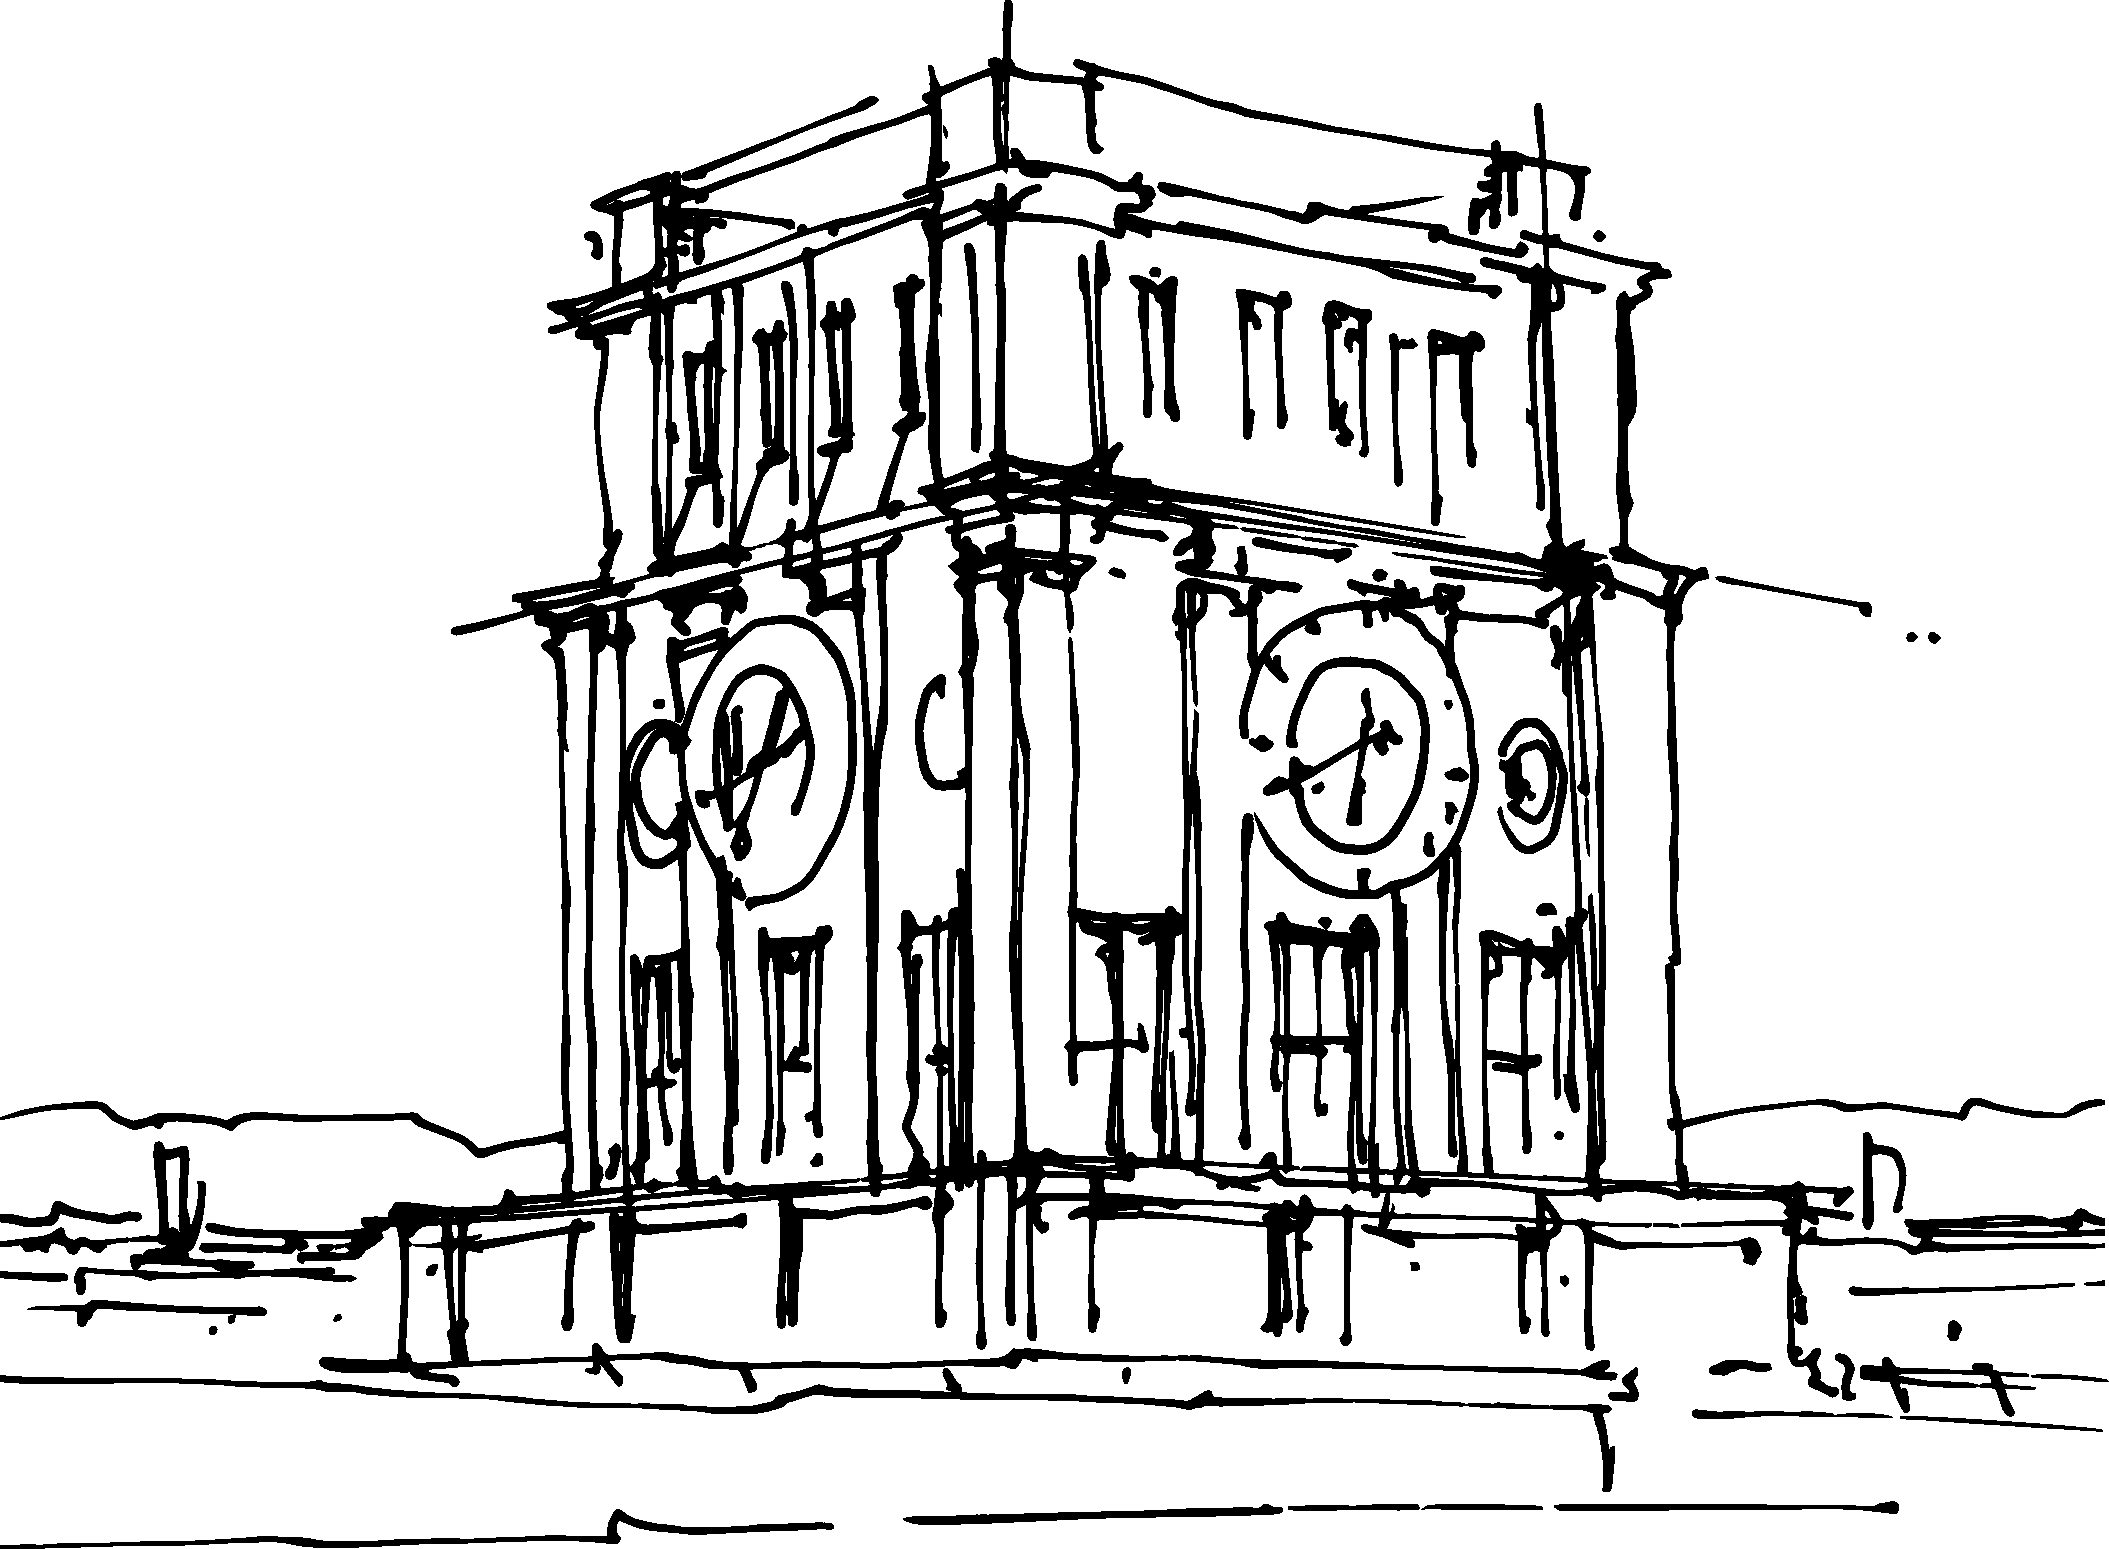
\includegraphics[width=9cm]{resources/TUM_Tower.pdf}}
  \caption{The TUM Tower in TUMBlue color.}
\end{figure}

\begin{figure}[h]
  \centering
  \textcolor{TUMWhite}{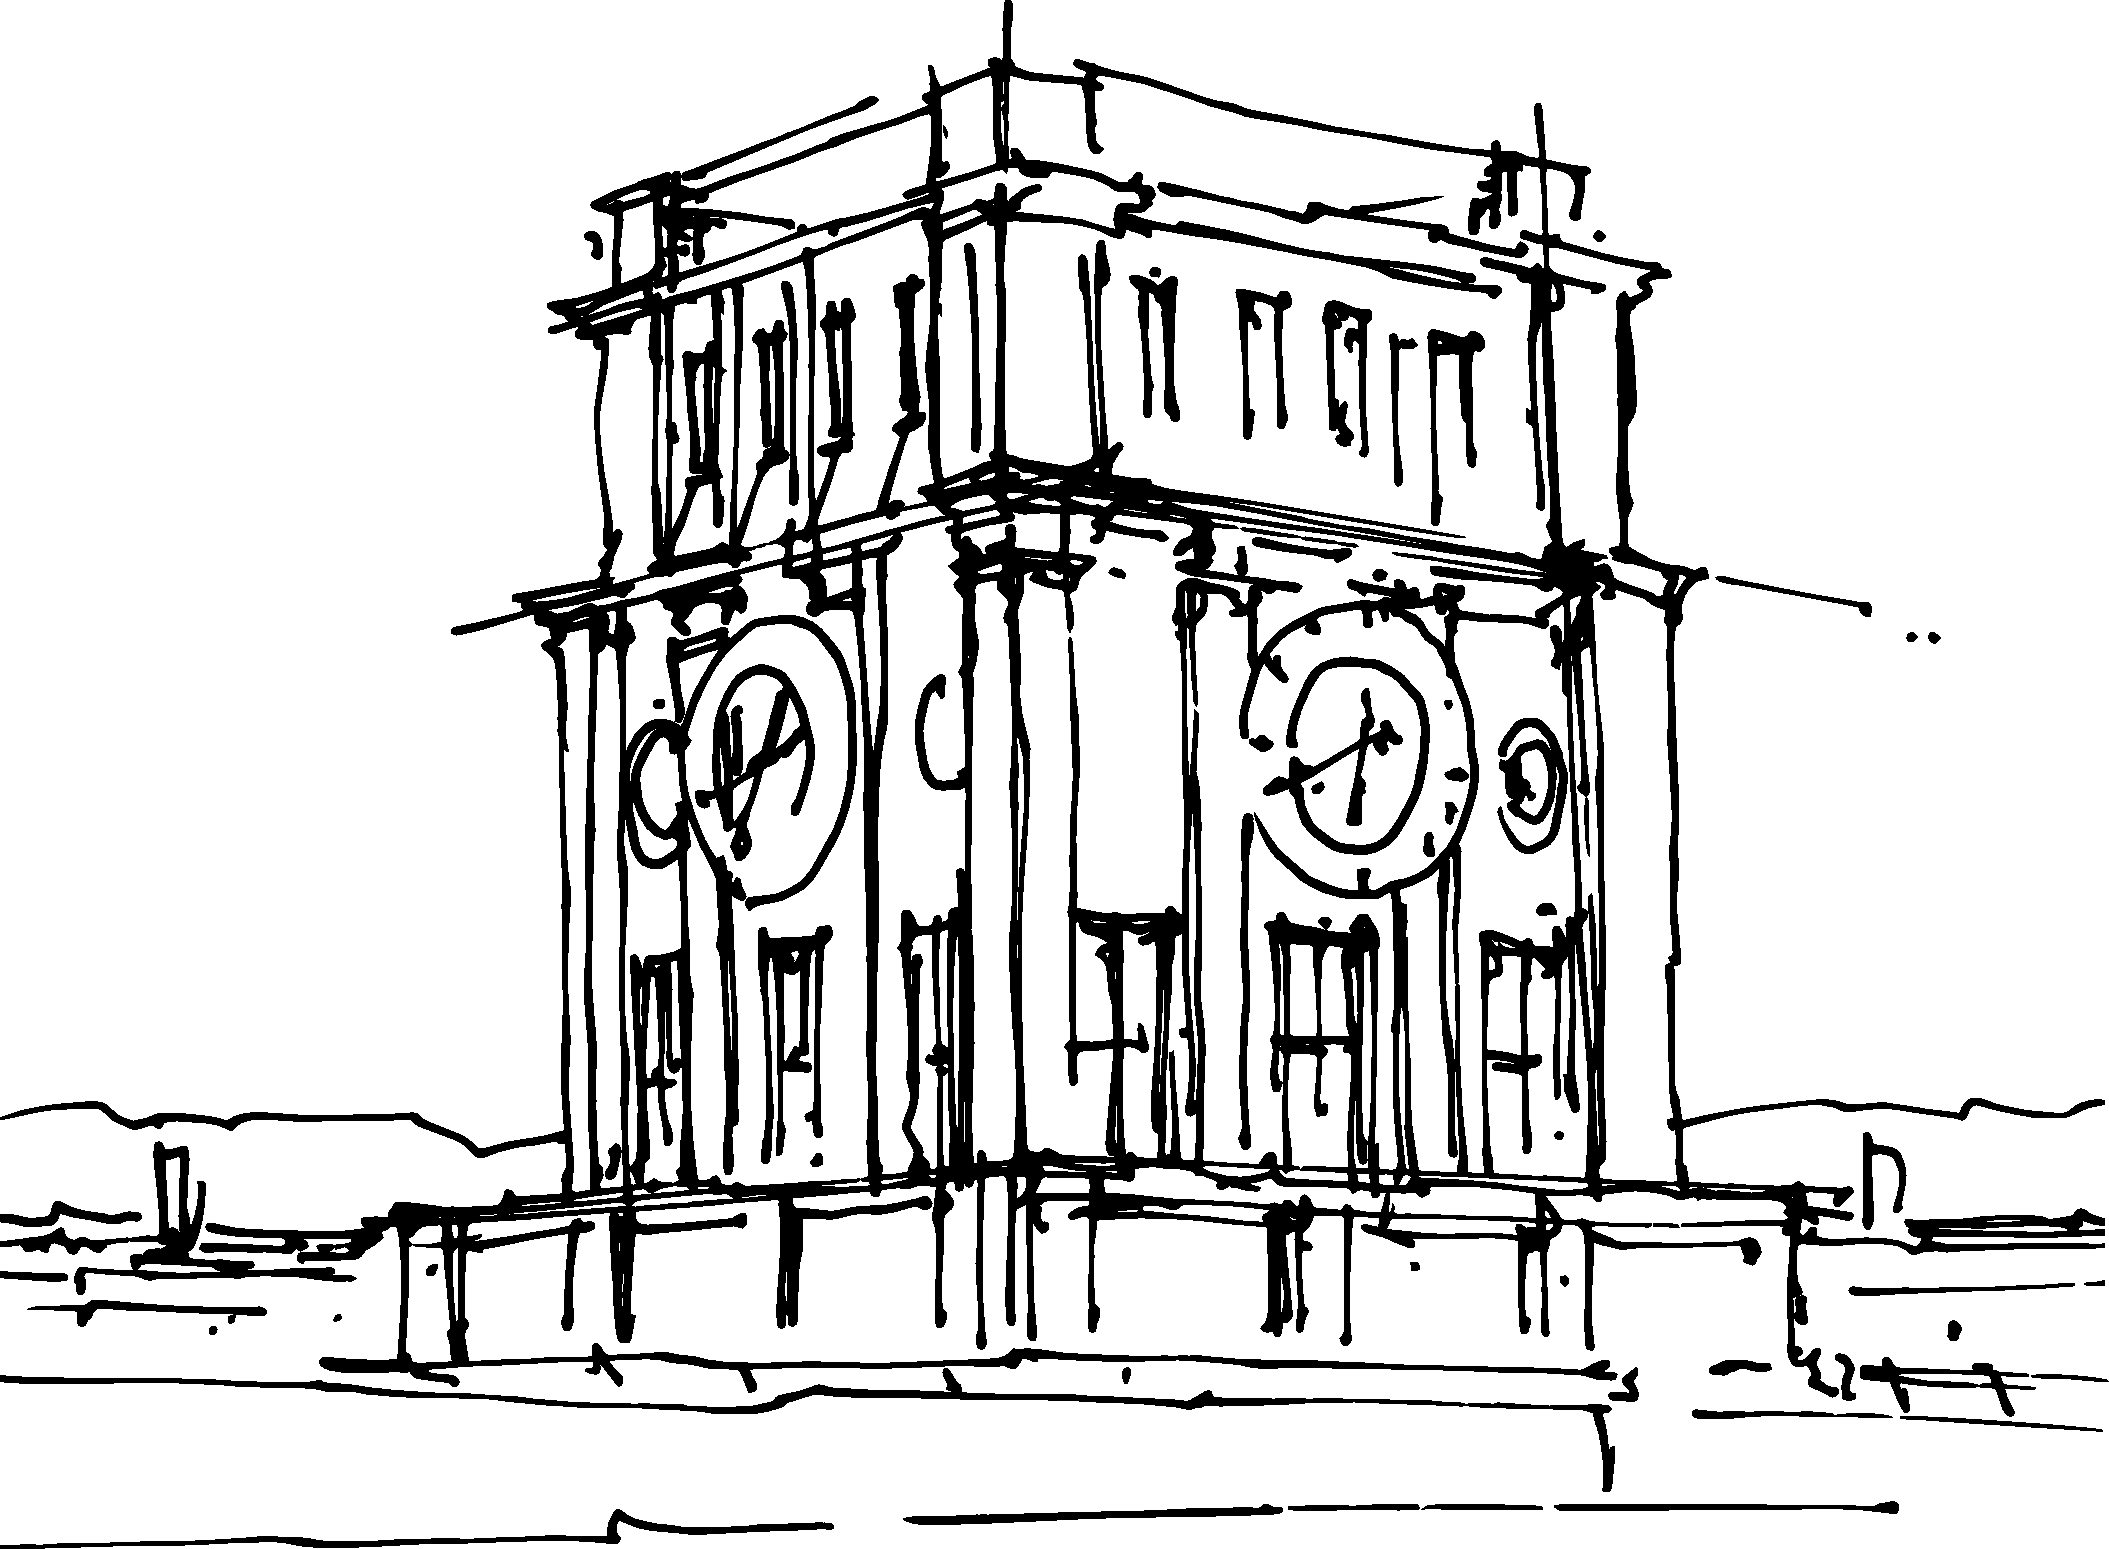
\includegraphics[width=9cm]{resources/TUM_Tower.pdf}}
  \caption{The TUM Tower in TUMWhite color.}
\end{figure}

\end{document}
